\scanpage{29}
Donc on a reconstruit les ens de sommets, d'arêtes, de faces de l'\uline{icosaèdre gauche} en termes de $(T,\unsure{\bar\omega|\varpi})$. Il faudrait reconstruire aussi les relations d'incidence.
\[
\begin{aligned}
\bar s\in\bar S&\longleftrightarrow\pi\in\mathrm{Pent}^+(T,\bar\omega)\\
\bar a\in\bar A&\longleftrightarrow\{\tau,\unsure{\gamma|\theta},\alpha\}\in\mathbb A^+(T,\bar\omega)\\
\bar f\in\bar F&\longleftrightarrow\deleted{\unsure{\{\omega,\omega'\}}}\ \Omega\in\unsure{\mathscr P|\mathfrak P}_2(T)
\end{aligned}
\]

\uline{Proposition}

a) $\bar s$ et $\bar a$ incidents sss $\gamma$ est la structure carrée sur $T\setminus\{\tau\}$ se déduisant de la structure pentagonale $\pi$ sur $T$ en prenant les sommets adjacents $u,v$ de $T$ à $t$, $\tilde u\ne\tau$ ($\tilde v\ne\tau$) adjacent à $u$, et la structure carrée de diagonales $\{u,\tilde u\},\{v,\tilde v\}$, donc \deleted{\unsure{$u\,v\,\tilde u\,\tilde v$}}
\diagram{\begin{tikzcd}[ampersand replacement=\&,row sep=small,column sep=small]
u\arrow[r,dash]\arrow[d,dash]\&v\\
\tilde v\arrow[r,dash]\&\tilde u
\end{tikzcd}}
, et $\alpha=\{\{u,v\},\{\tilde u,\tilde v\}\}$

\figure{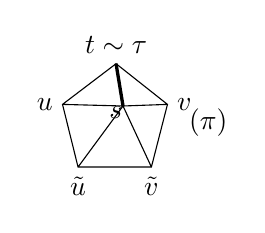
\begin{tikzpicture}[scale=.68]
\coordinate(t)at(0,1.1);\coordinate(u)at(-1,.34);\coordinate(v)at(.96,.34);
\coordinate(a)at(-.71,-.83);\coordinate(b)at(.66,-.83);\coordinate(s)at(.13,.31);
\draw (t)--(u)--(a)--(b)--(v)--cycle (u)--(s)--(v) (a)--(s)--(b);
\draw[very thick] (t)--(s);
\node[above]at(t){$t\sim\tau$};\node[left]at(u){$u$};\node[right]at(v){$v$};
\node[below]at(a){$\tilde u$};\node[below]at(b){$\tilde v$};
\node[below left,inner sep=0pt]at(s){$s$};\node[right]at(1.18,0){$(\pi)$};
\end{tikzpicture}}

\diagram{\begin{tikzcd}[ampersand replacement=\&,row sep=tiny,column sep=small]
\deleted{\unsure{\{s,u\}}}\arrow[r,dash]\&\deleted{\unsure{\{v,\tilde v\}}}\arrow[ddd,bend left]\\
\deleted{\{s,v\}}\arrow[r,leftrightarrow]\&\deleted{\{u,\tilde u\}}\\
\deleted{t}\&\deleted{\{t,u\}}\arrow[d,bend right,leftrightarrow]\\
\&\deleted{\{t,v\}}
\end{tikzcd}}

\diagram{\begin{tikzcd}[ampersand replacement=\&,row sep=tiny,column sep=small]
\{s,u\}\arrow[d]\&\\
\{s,v\}\arrow[d]\&\\
\{s,\tilde u\}\arrow[d]\&{\sim}\{t,v\}\\
\{s,\tilde v\}\arrow[uuu,bend left=48]\&{\sim}\{t,u\}
\end{tikzcd}}

[$\bar R=\vec A(\bar\Pi)$ s'identifie à l'ens des couples $(\pi,t)$, avec $\pi\in\mathrm{Pent}^+(T,\bar\omega)$, $t\in T$, donc $\bar R=\vec A(\bar\Pi)\simeq S(\bar\Pi)\times T\unsure{(\bar\Pi)}$

b) $\bar a$ et $\bar f$ sont incidents sss $\tau\in\underbrace{T\setminus\Omega}_{\unsure{\Phi''|\Phi}\deleted{\unsure{\varphi}}}$, \deleted{\unsure{$\mathrm{Alt}$}} $\gamma$ \inserted{sur $T\setminus\{\tau\}$} \deleted{\unsure{est défini}} par la condition que \inserted{$T\simeq\{\tau\}\amalg\bigl[\unsure{\Phi|\mathrm R}\setminus\{\tau\}\bigr]\amalg\Omega$}
\deleted{la relation ``ne pas être relié'' de}
\deleted{$\{T-\tau\}$ \unsure{est l'unique bijection|est l'unique bipartition} $\{\unsure{T|\Phi}-\tau\}$ et $\Omega$ telle que}
\deleted{\illegible{1}} 1°) $\unsure{\Phi|\mathrm R}-\tau$ et $\Omega$ sont des arêtes (opposées) \inserted{pour $\gamma$},
2°) et sont \deleted{\unsure{$\in$}} $\alpha$ (donc $\alpha$ est déterminé par $\gamma$ \unsure{l'est|l'étant}) \deleted{\unsure{et il y a a priori deux structures carrées possibles}}
\figure{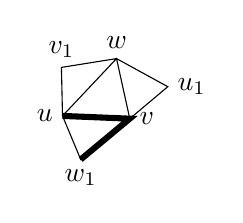
\begin{tikzpicture}[scale=.7]
\coordinate(a)at(-1,.88);\coordinate(w)at(0,1.04);\coordinate(b)at(.93,.53);
\coordinate(u)at(-.98,0);\coordinate(v)at(.24,-.05);\coordinate(c)at(-.65,-.79);
\draw (a)--(w)--(b)--(v)--(c)--(u)--cycle (u)--(w)--(v);
\draw[line width=2.2pt] (u)--(v)--(c);
\node[above]at(a){$v_1$};\node[above]at(w){$w$};\node[right]at(b){$u_1$};
\node[left]at(u){$u$};\node[right]at(v){$v$};\node[below]at(c){$w_1$};
\end{tikzpicture}}
\diagram{\begin{tikzcd}[ampersand replacement=\&,row sep=tiny]
\{u,w_1\}\arrow[d]\\
\{w_1,v\}\arrow[d]\\
\{v,w\}\arrow[d]\\
\{w,u\}\arrow[uuu,bend left=53]
\end{tikzcd}}
% archive sheet number: 28
